\section{Agent-server communication}
The vehicle needs a solid way of communicating with the server and other devices. 
We chose to use a server which hosts a REST API to achieve this. 
A REST API uses HTTP requests to communicate text strings in JSON format.
All actions are initiated by the clients, and the server is ``resting'' otherwise. 
A JSON object is a normal string, formatted in a certain way known by both end points.
This API is described in greater detail in the server section of this report.
The vehicle part of the communication was written in C++ to ensure compatibility with the other modules.
The following libraries were used:
\begin{itemize}
    \item Jansson - A library for processing JSON objects in C
    \item Curl - A library for making HTTP calls in C
\end{itemize}

\subsection{Sending and receiving commands}
Any client using this C++ framework for server communication can both receive commands from the server, and send commands to other client.
%TODO: Anders: What framework?
Commands are sent using the \textit{json\_send\_command} function.
It takes a command string as input, as well as the receiving client id for the command.
The \textit{json\_get\_commands} function provides a vector of command strings. It contains all the commands that were sent to your client id since the last time this function was called. 
It is up to the user to iterate trough this vector and extract the command strings, as well as perform action based on the commands received. 
We use commands like ``forward'',``backward'',``turn\_left'' and ``stop''.
It is up to the user what the various commands are, but both endpoints of communication must agree upon which commands are used.
The server will be ``stupid'' in this regard, as it only stores and send information when requested. 
All agents and users in the system can send commands to each other, unless access restrictions are implemented.

\subsection{Sending and receiving sensor data}
Sensor data is sent and received in a similar fashion as commands.
The vehicle code must construct a table of sensors and their associated sensor values. 
In practice this table is a C++ map. 
The vehicle passes this map into the \textit{json\_send\_data} function, which then constructs a JSON object containing all the data arranged in a predetermined structure. 
The JSON object is sent to the server using its REST API.
When a client wishes to get the latest sensor data from the vehicle, it simply calls the \textit{json\_get\_data} function.
It must specify which vehicle it wants to receive data from.
The function return a map of sensors to the client, identical to the one the vehicle uploaded.

\begin{figure}[H]
    \centering
    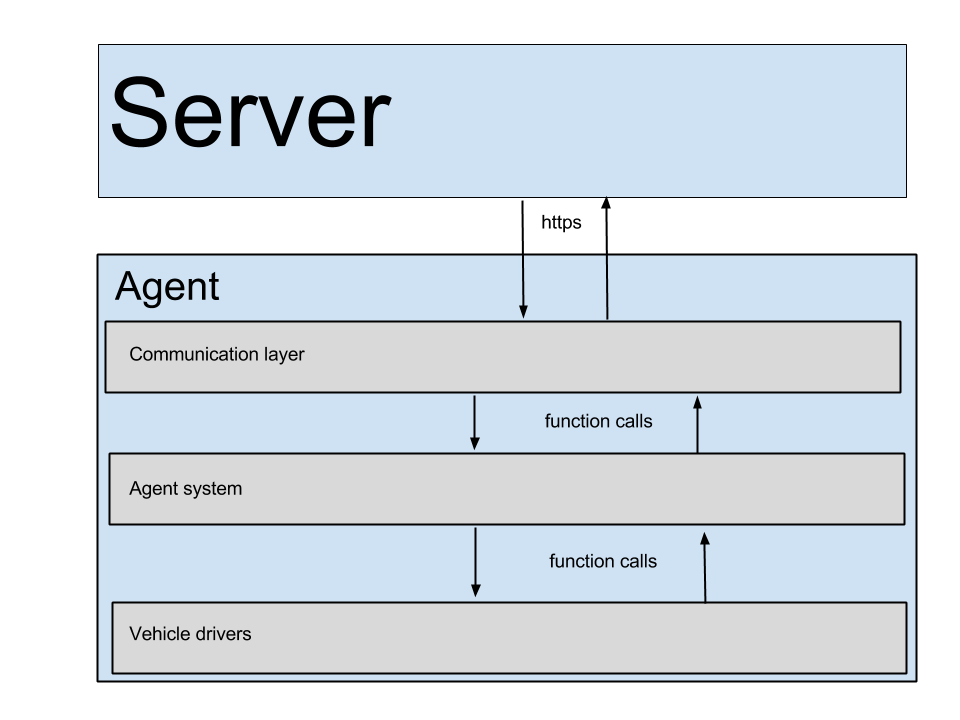
\includegraphics[width=0.7\textwidth]{graphics/Agent_server_communication.png} 
    \caption{Structure of server-agent communication}
    \label{fig:agent_server_communication}
\end{figure}

